

\chapter{Bewertungskriterien}
In diesem Kapitel werden die für eine Eignung bzw. Uneignung benötigten Kriterien vorgestellt.
Sie sollen helfen, eine Modellierungssprache zu bewerten. Dazu sind die Kriterien in Hauptkategorien untergliedert und werden im Verlauf weiter aufgelöst. 
Dabei handelt es sich um Eigenschaften und deren Ausprägung in einer Modellierungssprache.
Sie können auf die Modellierungssprache in ihrer Gesamtheit, aber auch auf einzelne Bestandteile oder Sprachmittel angewendet werden.
In vielen Fällen bestehen zwischen den einzelnen Eigenschaften enge Beziehungen.
Je nachdem für welchen Sprachbestandteil die Bewertung vorgenommen wird, können andere Maße für die Bewertung verwendet werden.
Für viele der hier vorgestellten Merkmale gibt es jedoch keine exakten Bewertungsverfahren, inwieweit das Merkmal erfüllt ist oder nicht.
Die Kriterien sind in drei Kategorien eingeteilt, auf welche im Folgenden eingegangen wird:

\begin{itemize}
		\item Formale Kriterien
		\item Anwenderbezogene Kriterien
		\item Anwendungsbezogene Kriterien
\end{itemize}

\section{Formale Kriterien}  
Die formalen Kriterien werden in die fünf Einzelkriterien Korrektheit, Vollständigkeit, Einheitlichkeit, Redundanzfreiheit und Strukturierbarkeit unterteilt.
\subsection{Korrektheit}
Eine Modellierungssprache genügt dem Kriterium der Korrektheit, wenn sie unzulässige Modelle eindeutig identifiziert und gleichzeitig erlaubt, die Menge aller zulässigen Modelle zu generieren. Zu unterscheiden ist dabei die syntaktische Korrektheit sowie die semantische Korrektheit der Modelle. Die semi-formalen Prozessmodellierungssprachen, welche für die Prozessdokumentation in Frage kommen, besitzen in der Regel keine eindeutig festgelegte Semantik, sodass hier vor allem die Möglichkeit der automatischen Überprüfung einer korrekten Syntax des Modells im Vordergrund steht. Das Kriterium der Korrektheit steht in enger Verbindung zum Grundsatz der Richtigkeit der Grundsätze ordnungsgemäßer Modellierung.
\subsection{Vollständigkeit}
Unter Vollständigkeit wird in diesem Zusammenhang die Vollständigkeit der Sprachbeschreibung verstanden. Alle Konstrukte sowie die Bedingungen ihrer Verwendung, die von der Modellierungssprache bereitgestellt werden, müssen eindeutig definiert und beschrieben sein (Süttenbach und Ebert 1997, S. 3).
\subsection{Einheitlichkeit}
Das Kriterium der Einheitlichkeit ist angelehnt an den Grundsatz der Klarheit der GoM. Einheitlichkeit bedeutet in diesem Kontext, dass alle Konstrukte der Sprache verständlich dargestellt und beschrieben werden. Ähnliche Konstrukte sollten somit auch in ähnlicher Weise spezifiziert werden.
\subsection{Redundanzfreiheit}
Die Redundanzfreiheit setzt voraus, dass die Sprache keine Mehrfachdefinition von Konstrukten vornimmt, die denselben Sachverhalt beschreiben. Ein und derselbe Sachverhalt sollte also nicht mit mehreren verschiedenen Elementen bzw. Symbolen der Modellierungssprache belegt sein. Auch dieses Kriterium fördert den Grundsatz der Klarheit. Indem gleiche realweltliche Sachverhalte in der Modellierungssprache durch gleiche Konstrukte ausgedrückt werden, wird zudem der Grundsatz der Vergleichbarkeit gefördert.
\subsection{Strukturierbarkeit}
Da Informationsmodelle eine hohe Komplexität aufweisen können, sollte die Sprache Konstrukte bereitstellen, welche die Strukturierung der modellierten Informationen unterstützt. Die Modellierungssprache muss also Zerlegungen in Prozesskomponenten oder Teilprozesse darstellen können. Die Schnittstellen zwischen den Komponenten müssen übersichtlich dargestellt werden. Verallgemeinerungen (Generalisierung) und Detaillierungen (Spezialisierung) müssen schlüssig nachvollziehbar sein. Die Strukturierung in Teilmodelle ermöglicht gleichzeitig die Wiederverwendbarkeit der Strukturen in anderen Modellen. So können etwa modellierte Teilprozesse in anderen Prozessen wieder aufgegriffen werden und müssen nicht mehrfach modelliert werden. Zusätzlich wird dadurch die Wartbarkeit der Modelle verbessert, da Änderungen in einem Modellteil, die Konsistenz der übrigen Modellteile nicht beeinflussen. Das Kriterium der Strukturierbarkeit unterstützt den Grundsatz des systematischen Aufbaus der Grundsätze ordnungsgemäßer Modellierung


\section{Anwenderbezogene Kriterien}
Modellierungssprachen bieten die Möglichkeit, Ideen und Gedanken mittels Modelle austauschen zu
können. Modellierungssprachen sind Sprachen, die primär für menschliche Anwender als Mittel zur
Kommunikation bestimmt sind. Die anwenderbezogenen Kriterien beleuchten dieses Verhältnis zwischen
Modellierungssprache und Anwender.
Die anwenderbezogenen Kriterien beschreiben das Verhältnis zwischen dem Anwender und der verwendeten Modellierungssprache. Der Anwender kann zum einen der Modellierer und zum anderen der Betrachter eines Modells sein. Die anwenderbezogenen Kriterien besitzen eine besondere Bedeutung, um Nutzern von Modellen das Verständnis zu erleichtern bzw. zu ermöglichen. Für den betrachteten Anwendungsfall der Prozessdokumentation, zur Nutzung als allgemeine Arbeitsgrundlage für die Mitarbeiter einer Organisation, spielen sie daher eine sehr große Rolle. Die Modellierungssprache ermöglicht das Erstellen von Modellen, um Ideen und Gedanken zwischen den Beteiligten auszutauschen. Sie sind somit in erster Linie für den menschlichen Anwender als Kommunikationsmittel zu verstehen.  
\subsection{Anschaulichkeit und Verständlichkeit}
Hier geht es einerseits um eine dem Modellbegriff schon fast inhärente Forderung: Ein Modell sollte
anschaulich sein. Andererseits ist hier an den Umstand zu denken, dass Modelle der Abbildung faktischer
oder geplanter Realität dienen. Solche Abbildungen können grundsätzlich fehlbar sein. Ein
Modell sollte seine Überprüfung an der Realität unterstützen. \\

Ein Modell ist dann anschaulich, wenn es möglichst direkt mit Wahrnehmungsmustern und Konzeptualisierungen
des Betrachters korrespondiert. Wahrnehmungsmuster und Konzeptualisierungen
streuen aber bekanntlich interpersonell und intrapersonell (der Mensch ist lernfähig). Anschaulichkeit
in diesem Sinn hängt einerseits den jeweils gewählten Abstraktionen und Bezeichnern ab, andererseits
von der jeweiligen Modellierungssprache (worauf noch einzugehen sein wird). Die Beurteilung der
Beziehung zwischen Modell und Realität liegt in der Regel allein bei den Betrachtern. Die Anschaulichkeit
eines Modells ist also grundsätzlich geeignet, seine Überprüfbarkeit zu fördern. Dabei ist es wesentlich,
dass das Verhältnis des Modells zur Realität durch möglichst genaue Abbildungsvorschriften
erläutert wird. \\
\subsubsection{Konsequenzen für Modellierungssprachen} 
Da Wahrnehmungsmuster und Konzeptualisierungen weit und in subtiler Weise streuen, sind generelle
Aussagen über die Wirkung einer Modellierungssprache auf die Anschaulichkeit eines Modells kaum
möglich. Allgemein lässt sich vermuten, dass Syntax und Semantik einer Modellierungssprache tendenziell
dann als anschaulich empfunden werden, wenn sie eine deutliche Nähe zu Sprachmitteln aufweisen,
die der jeweilige Betrachter aus ihm vertrauten Sprachen kennt - also beispielsweise das generelle
Muster "Subjekt, Prädikat, (Objekt)". Der Stand der Forschung in diesem Bereich muss allerdings als
unbefriedigend angesehen werden. Es gibt nur wenige empirische Untersuchungen, die die Anschaulichkeit
von konzeptuellen Modellen aus der Sicht verschiedener Betrachter zum Gegenstand haben (so
etwa [GoSt90], [Hit95]). Dabei hat sich gezeigt, dass viele Betrachter erhebliche Schwierigkeiten hatten,
die ihnen vorgelegten Modelle nachzuvollziehen. Ein solches Ergebnis kann kaum überraschen:
Schließlich wurden Modellierungssprachen in der Regel nicht nach den Wünschen möglicher Anwender entworfen.
Wir können an dieser Stelle lediglich zweierlei festhalten: Je mehr Diagrammarten geboten
werden, desto größer die Wahrscheinlichkeit, dass eine Diagrammart im Kreis der Betrachter intuitiv
verstanden wird. Je stärker eine Diagrammart die spezifischen Besonderheiten einer Domäne berücksichtigt,
desto größer ist die Wahrscheinlichkeit, dass die Kenner dieser Domäne entsprechende Diagramme
für anschaulich halten. Anschaulichkeit impliziert sinnvollerweise das Verstehen der verwendeten
Modellierungssprache. Das empfiehlt die Forderung nach leichter Erlernbarkeit: Je geringer die
Zahl der Modellierungskonzepte und je einfacher die zu berücksichtigenden Verknüpfungsregeln,
desto leichter ist eine Sprache zu erlernen. Dabei muss allerdings berücksichtigt werden, dass diese
Anforderung ggfs. im Konflikt mit dem Bemühen um Anschaulichkeit steht.\\
\subsubsection{Feststellbarkeit/Meßbarkeit der Beurteilungskriterien} 
Auch wenn Modellierungssprachen unzweifelhaft einen erheblichen Einfluss auf die Anschaulichkeit
von Modellen haben, ist uns die Erfassung und Beurteilung dieses Einflusses in befriedigender Weise
nicht möglich. Wir können lediglich auf einige Indikatoren hinweisen. Die verschiedenen Diagrammarten
verbessern tendenziell die Chance, individuell als anschaulich empfundene Sichten zu befriedigen.
Diesem Vorteil steht allerdings ggfs. der Nachteil redundanter Sprachelemente gegenüber,
wodurch die Erlernbarkeit der gesamten Sprache verschlechtert wird. Weiterhin sind domänenspezifische
Diagrammarten geeignet, Anschaulichkeit für bestimmte Betrachtergruppen zu fördern. Als Beispiel
sei eine Diagrammart zur Abbildung von Geschäftsprozessen im Rahmen der Entwicklung
betrieblicher Informationssysteme genannt.
\\
Darüber hinaus sind Symbole zur Kennzeichnung ergänzender Kommentare wünschenswert. Die
Erlernbarkeit einer Sprache wird durch die Dokumentation erleichtert. Neben der verständlichen
Beschreibung der Sprachkonzepte ist hier an die Erläuterung der Verwendung der Sprache zu denken -
ggfs. durch Beispiele ergänzt.\\
Auch die Verständlichkeit der Sprache wirkt sich direkt auf die Anschaulichkeit der Sprache aus. Die
Verwendung der einzelnen Sprachmittel sollte klar festgelegt sein, und es sollten Entscheidungshilfen
bei Alternativen gegeben werden. Auch die Eindeutigkeit der Semantik der Sprachmittel ist eine wichtige
Voraussetzung für eine verständliche Sprache.\\

\subsection{Angemessenheit}
Das Kriterium der Angemessenheit steht in direktem Zusammenhang mit der Mächtigkeit und dem
Anwendungszweck einer Sprache. Die Angemessenheit ist immer relativ zum Anwendungszweck zu
sehen. Sie bezieht sich sowohl auf die Sprache in ihrer Gesamtheit als auch auf die einzelnen Sprachkonzepte.
Angemessenheit und Mächtigkeit bieten zusammen die Möglichkeit, zu untersuchen, ob
eine Sprache für den Anwendungszweck ausreichende Konzepte bereitstellt, gleichzeitig aber keine
überflüssigen Konzepte enthält.
\subsubsection{Konsequenzen für Modellierungssprachen}
Insbesondere bei sehr speziellen Sprachkonstrukten muß untersucht werden, ob diese Konstrukte nötig
sind oder ob sie nur zu einer Erhöhung der Sprachkomplexität führen. Die Entscheidung, ob ein
Sprachmittel angemessen ist oder nicht, ist jedoch häufig nicht objektiv vornehmbar, sondern hängt
stark von den Präferenzen der jeweiligen Betrachter ab. Im allgemeinen gibt es immer Vor- und Nachteile
für einzelne Sprachmittel, so dass ein sorgsames Abwägen notwendig ist.
\subsubsection{Feststellbarkeit/Meßbarkeit der Beurteilungskriterien} 
Generelle formale Maße zur Bestimmung der Angemessenheit von Modellierungssprachen gibt es
nicht. Die Untersuchung der Angemessenheit eines Sprachelementes kann daher nur subjektiv erfolgen.
Dabei ist zu untersuchen, ob ein Sprachelement bedeutsam für den Anwendungszweck ist oder
nicht.
\subsection{Überprüfbarkeit}
Modelle dienen der Abbildung faktischer oder geplanter Realität. Solche Abbildungen können grundsätzlich
fehlbar sein. Ein Modell sollte seine Überprüfung an der Realität unterstützen. Der Einfluss der
Modellierungssprache auf die Überprüfbarkeit eines Modells ist ambivalent. So geht es einerseits
darum, eine möglichst genaue, intersubjektiv nachvollziehbare Überprüfung an der Wirklichkeit anzustreben.
Andererseits ist zu berücksichtigen, dass solche objektivierten Verfahren nicht für alle Facetten
eines Modells anwendbar sind und sich Modelle oft nicht auf faktische, sondern geplante Realität
beziehen. In diesen Fällen erfolgt die Überprüfung allein durch die Einschätzung der Betrachter. Idealtypisch
ist ein Modell dann als realistisch (im Hinblick auf Erwartungen) anzusehen, wenn im Kreise
gutwilliger und sachkundiger Betrachter ein Konsens darüber erzielt wurde. Während die objektivierte
Überprüfung eines Modells an der Realität tendenziell zur Forderung nach formalen Modellierungssprachen
führt, ergeben sich aus dem Bemühen um Konsensbildung andere Konsequenzen: Bekanntlich
fördert Mehrdeutigkeit die Chance, einen Konsens zu erzielen. Ein Modellierungsansatz wie die
"Soft System Methodology" ([Che81]) lässt den Betrachtern eben wesentlich mehr individuelle Interpretationsspielräume
als eine Sprache zur formalen Systemspezifikation. Wegen dieser widersprüchlichen
Konsequenzen ist das Kriterium "Überprüfbarkeit" nicht zur Diskriminierung zwischen Modellierungssprachen
geeignet.\\
Ein Modell ist eine vereinfachte und idealisierte Abbildung eines Problembereichs. Im Modell werden
nur die für die Betrachtung wesentlichen Eigenschaften berücksichtigt und unwesentliche vernachlässigt.
In Abb.  ist die Beziehung zwischen Modell und zu modellierendem Sachverhalt dargestellt.
\begin{center}
\begin{figure}[h]
   

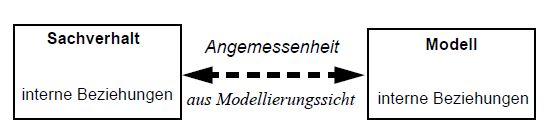
\includegraphics[scale=1]{Graphics/Sachverhalt.jpg}

\captionof{figure}{Beziehung zwischen Modell und zu modellierendem Sachverhalt }


Quelle : EIN BEZUGSRAHMEN ZUR BEURTEILUNG OBJEKTORIENTIERTER MODELLIERUNGSSPRACHEN - VERANSCHAULICHT AM BEISPIEL VON OML UND UML , ULRICH FRANK und MICHAEL PRASSE
 

 
\label{fig9}


\end{figure}

\end{center}

Modelle bedürfen immer der Überprüfung mit dem zu modellierenden Sachverhalt. Zwischen Sachverhalt
und Modell existiert immer eine Beziehung, die ein Maß für die Angemessenheit des Modells ist.
Die Bewertung der Angemessenheit eines Modells kann nur relativ zum Modellierungszweck erfolgen,
da Modelle von unwesentlichen Details abstrahieren. Im allgemeinen kann diese Beziehung nicht
direkt angeben werden, da der Sachverhalt meistens nur unklar spezifiziert ist1. Aus diesem Grund ist
es auch nicht möglich, immer automatisch zu überprüfen, ob ein Modell den gewünschten Sachverhalt
modelliert. Nur wenn der Sachverhalt selbst als exakte Beschreibung2 vorliegt und auch das Modell
exakt beschrieben ist, wird ein formales Überprüfen erst möglich, und die Angemessenheit eines
Modells kann formal bewertet werden. Meistens ist der Sachverhalt jedoch nicht klar spezifiziert.\\
Die einzige Möglichkeit ist dann, den Inhalt des Modells zu erfassen und zu überprüfen, ob dieser mit
dem zu modellierenden Sachverhalt übereinstimmt. Je exakter und präziser ein Modell interpretiert
werden kann, desto leichter kann es mit dem zu modellierenden Sachverhalt verglichen werden.
Obwohl es nicht möglich ist, die Adäquanz zwischen einer eventuell unpräzisen Darstellung (Sachverhalt)
und einer möglichst präzisen Darstellung (Modell) prinzipiell zu entscheiden, hilft eine präzise
Darstellung und eindeutige Interpretation des Modells beim Vergleich mit dem zu modellierenden
Sachverhalt. Eine Modellierungssprache, die es ermöglicht, Modelle exakt und eindeutig zu beschreiben
und zu interpretieren, erleichtert daher wesentlich die Überprüfung des Modells.\\
Nur wenn Modelle eindeutig sind, ist eine korrekte Verständigung möglich. Dies verlangt eine eindeutige
Interpretation der einzelnen Sprachmittel und Regeln zur syntaktischen Verknüpfung dieser
Sprachmittel. Andernfalls bieten sich Interpretationsfreiräume, die zu Missverständnissen führen können.
Die exakte Festlegung der abstrakten Syntax und Semantik der Sprache ist somit Voraussetzung
für die eindeutige Interpretierbarkeit der Modelle. Beim Betrachten eines Artefakts der Modellierungssprache
hat man im allgemeinen nicht wie bei Programmen die Möglichkeit, durch Inspizieren oder
Ausprobieren des Codes die Aufgabe der Software herauszubekommen. Vielmehr ist die Beschreibung
der Metasprache die einzige Referenz.\\
Ein anderer Aspekt der Überprüfung betrifft die Nachvollziehbarkeit und Rückverfolgung von Modellierungsentscheidungen.\\
\subsection{Mächtigkeit}
Die Mächtigkeit einer Modellierungssprache bezieht sich unter anderem auf die Ausdrucksmächtigkeit
der bereitgestellten Konzepte. Eine Modellierungssprache sollte sich auf die Modellierung konzentrieren.
So können zu viele Konzepte zu einer unangemessen mächtigen Sprache führen. Zwischen Mächtigkeit
und Angemessenheit muss daher ein ausgewogenes Verhältnis existieren.\\
Mächtigkeit kann aber auch relativ zur Mächtigkeit von Turingmaschinen betrachtet werden und ist
dann ein Maß für die Berechnungsfähigkeit einer Modellierungssprache. Für Modellierungssprachen
ist diese Betrachtung jedoch nicht ganz korrekt, da sie im allgemeinen keine Formalisierungen von
Algorithmen sind.
\subsubsection{Konsequenzen}
Mächtigkeit und Angemessenheit bedingen einander. Die Mächtigkeit einer Sprache muss daher relativ
zum Anwendungsbereich betrachtet werden. Geht man grundsätzlich davon aus, dass die hier betrachteten
Modellierungssprachen der konzeptuellen Modellierung dienen, misst sich die Mächtigkeit einerseits
an der Möglichkeit, als wesentlich erkannte Sachverhalte des abzubildenden Realitätsbereichs
natürlich, also ohne aufwendige Rekonstruktionen, beschreiben zu können. Andererseits sollte die
Modellierungssprache auch Möglichkeiten bieten, Informationen darzustellen, die für die Implementierung
benötigt werden.


